%!TEX root=../document.tex

\section{Ergebnisse}
\label{sec:Ergebnisse}

\subsection{Theoretische Fragestellungen}
\subsubsection{Nutzung von GPUs in normalen Desktop-Anwendungen}
\textbf{Einführung}\\
Die Nutzung von GPUs in Desktop-Anwendungen ist meistens unter dem Begriff ''Hardware acceleration'' (Hardwarebeschleunigung) bekannt.\\
Hardwarebeschleunigung entlastet die CPU durch Delegation rechenintensiver Aufgaben an für diese Aufgaben optimierte Hardware. In den meisten Fällen ist dies die GPU. \cite{hardwareacc_streamingmedia} \\\\
Der Vorteil von GPUs gegenüber CPUs ist die Nebenläufigkeit. CPUs sind sequentiell ausführende Prozessoren, während GPUs auf nebenläufige Ausführung spezialisiert sind. \cite[S. 2-3]{programminggpgpu_kirk} \\
Für bestimmte, rechenintensive Aufgaben ist es daher sinnvoll, die GPU anstelle der CPU zu verwenden. Allerdings sollte beachtet werden, dass die Delegation an die GPU durchaus aufwändig sein kann.\\
Beispielsweise ist das Kopieren von Ressourcen ein Faktor, welcher berücksichtigt werden sollte.\\\\
\textbf{Anwendungen}\\
Hier einige Anwendungen, welche Programmteile auf der GPU ausführen:
\begin{itemize}
\item Microsoft Office
\item VLC
\item Verschiedene Browser (Besonders für HTML5)
\end{itemize}
Zusätzlich ist es meistens möglich, die Hardwarebeschleunigung manuell ein- bzw. auszuschalten.
\newpage
\subsubsection{IDEs und Programmiersprachen}
\textbf{OpenCL}\\
Eine OpenCL-Applikation besteht aus 2 Bestandteilen - dem Host und den ''Compute Devices''. Die Compute-Devices stellen CPUs, GPUs oder andere Prozessortypen dar. Auf den Devices findet die eigentliche Berechnung statt. Der Host ist dafür zuständig, die Aufgaben an die Devices zu verteilen. \cite{openclprogramming_munshi} \\\\
Der Host-Code kann dabei in verschiedenen Programmiersprachen wie C++ oder Java programmiert werden. Der Code für die Compute-Devices (Kernels) wird allerdings in der OpenCL Programming Language, auch OpenCL C genannt, programmiert. \cite{openclprogramming_munshi}\\\\
Als Entwicklungsumgebung kann eine beliebige IDE für die jeweilige Sprache genutzt werden. Um besondere Funktionen für die nebenläufige Programmierung zu nutzen, bietet OpenCL \\''OpenCL Studio'' an. \cite[S. 12]{openclstudio} \\\\
\textbf{CUDA}\\
Eine CUDA-Anwendung besteht ebenfalls aus einem Host und mehreren Devices. Der Device-Code wird dabei ebenfalls in einer C-ähnlichen Sprache verfasst. Für den Host-Code existieren ebenfalls diverse Bindings. \cite[S. 41]{programminggpgpu_kirk} Als speziell angepasste ''IDE'' stellt Nvidia das Nsight Eclipse Plugin zur Verfügung. \cite{nsighteclipse}

\subsubsection{Bestehende Programme auf GPUs nutzen}
Prinzipiell ermöglichen es bestimmte Tools, bestehenden Code in OpenCL zu übersetzen. Allerdings können die Ergebnisse wenig zufriedenstellend ausfallen. In den meisten Fällen ist es sinnvoller, den OpenCL C Code selber zu schreiben. Dies macht es möglich, den Code entsprechend zu parallelisieren und zu optimieren. Das Übersetzen von bestehendem Code in OpenCL C ist oft nicht ausreichend um eine Performanceoptimierung zu erzielen.\\\\
\textbf{Aparapi}\\
Aparapi ist ein Tool, dass Java Bytecode während der Laufzeit in OpenCL C übersetzt und auf der GPU ausführt. Wenn die Übersetzung wegen eines Fehlers nicht möglich ist wird der Code in Thread Pools auf der CPU ausgeführt.\cite{aparapi}

\newpage

\textbf{CUDA LLVM Compiler}\\
CUDA LLVM Compiler ist ein Backend für LLVM, dass LLVM IL (Intermediate Language) für eine Nvidia GPU kompiliert. So können eigene LLVM Frontends entwickelt werden, die GPU Beschleunigung mit CUDA unterstützen.

\begin{figure}[!h]
	\begin{center}
		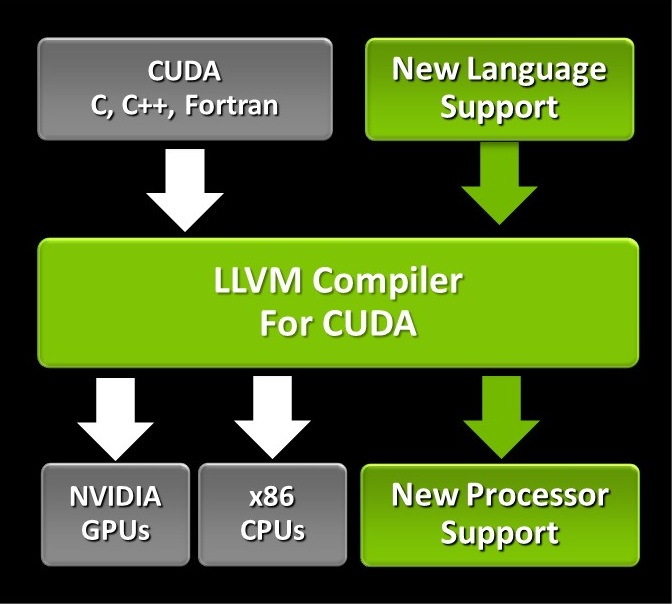
\includegraphics[width=7.5cm]{images/LLVM_Compiler_structure.jpg}
		\caption{CUDA LLVM Compiler Structure\cite{cudallvm}}
	\end{center}
\end{figure}

\textbf{Rootbeer GPU Compiler}\\
Mit Rootbeer GPU Compiler können Teile von Java Programmen auf einer GPU ausgeführt werden. Dabei wird zur Compile Time Java Bytecode für die GPU mithilfe von CUDA übersetzt. Während der Runtime wird der übersetzte Code ausgeführt.\cite{rootbeer1}

\subsubsection{Transcompiler}
Ein Transcompiler übersetzt Source Code von einer Sprache in eine andere.

\textbf{Swan}\\
Swan ist ein Tool um CUDA Kernel Sourcecode in OpenCL Sourcecode zu übersetzen. Nebenbei bietet es auch eine gemeinsame API um CUDA und OpenCL zu abstrahieren.\cite{swan}
\newpage
\subsection{Systemdaten}
Das folgende System wurde für die unten angeführten Benchmarks verwendet.
\subsubsection{Allgemein}
\begin{itemize}
\item Intel Core i7-3635QM CPU 2.40GHz
\item 8 GB DDR3-RAM
\item Samsung MZ-75E500B/EU 850 EVO 2,5 Zoll 500GB SSD (SATA III)
\item Windows 10 Pro 64-Bit
\item AMD Radeon R9 M200X Series 2048 MB
\end{itemize}
\subsubsection{CPU}
\begin{figure}[!h]
	\begin{center}
		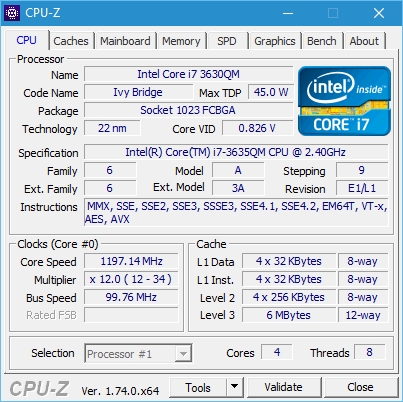
\includegraphics[width=10cm]{images/cpu_specs.png}
		\caption{CPU-Eigenschaften}
	\end{center}
\end{figure}
\newpage
\subsubsection{GPU}
\begin{figure}[!h]
	\begin{center}
		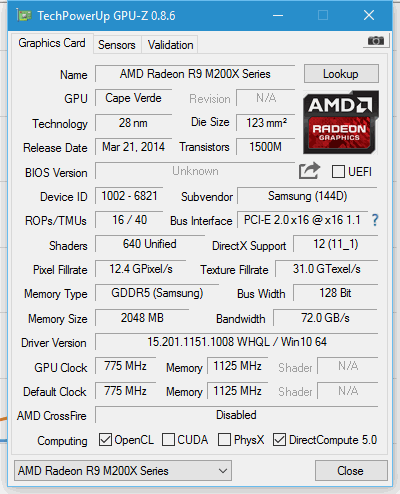
\includegraphics[width=10cm]{images/gpu_specs.png}
		\caption{GPU-Eigenschaften}
	\end{center}
\end{figure}
\newpage
\subsection{Bruteforce}
\subsubsection{Beschreibung}
Mithilfe von einer Brutforce Attacke wird versucht ein MD5 verschlüsseltes Passwort zu finden. Die Passwörter werden direkt auf der GPU generiert, gehasht und verglichen. So findet für die eigentliche suche das Passwortes keine Kommunikation zwischen CPU und GPU statt, womit der PCI Bus als Bottleneck ausgeschlossen werden kann.
\subsubsection{Ausführen des Programmes}
Das fertige Projekt inklusive \texttt{pom.xml} befindet sich im ZIP-File. Zum Builden der JAR kann \texttt{mvn clean install} ausgeführt werden. Das JAR-File namens \texttt{dezsys08-gpgpu-1.0.0.jar} befindet sich dann im \texttt{target} Verzeichnis. Zum Ausführen muss in der Konsole folgender Befehl ausgeführt werden:
\begin{center}
\texttt{java -jar dezsys08-gpgpu-1.0.0.jar}
\end{center}
Mit diesem Befehl wird die GPU zur Ausführung verwendet. Wenn der Parameter \texttt{cpu} hinzugefügt wird, wird die CPU verwendet. In diesem Zustand wird das Programm 8 mal ausgeführt, für den Benchmark wurden jedoch 100 verwendet. Um diese Anzahl anzupassen, muss die Variable \texttt{ITERATIONS} in der \texttt{Main}-Klasse auf den gewünschten Wert gesetzt werden. \\\\
Während der Ausführung wird für jeden Durchlauf die benötigte Zeit in der Konsole ausgegeben. Die einzelnen Ergebnisse befinden sich in der Datei \texttt{benchmark.ods}, für das Diagramm wurde jedoch der Mittelwert der 100 Werte berechnet.
\newpage
\subsubsection{Durchführung}
Es wurden jeweils 100 Durchläufe durchgeführt.
Die Ergebnisse sehen folgendermaßen aus:
\begin{figure}[!h]
	\begin{center}
		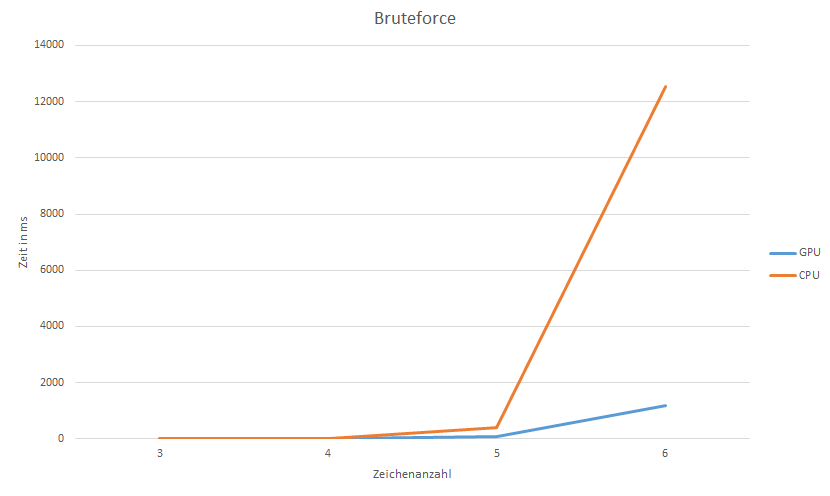
\includegraphics[width=17cm]{images/bruteforce.png}
		\caption{Bruteforce-Benchmark}
	\end{center}
\end{figure}
\subsubsection{Fazit}
Dieser Algorithmus kann gut parallelisiert werden, da die Arbeit in kleine Pakete aufgeteilt werden kann. Jedes dieser Pakete wird unabhängig von einander bearbeitet. Hierbei muss keine Kommunikation zwischen Host Code und Kernel stattfinden, was zusätzlich die Performance erhöht. Weil dieser Algorithmus so gut parallelisiert bar ist und wenig Kommunikation zwischen Host und Kernel stattfindet ist die GPU im Vorteil. Aber erst bei einer Wortlänge von 6 ist die GPU um 1 Magnitude schneller.

\newpage
\subsection{GPUPI}
\subsubsection{Beschreibung}
GPUPI berechnet PI mithilfe der BPP (Bailey-Borwein-Plouffe) Formel. Dieser Benchmark hängt vor allem von der 64 Bit Integer Performance ab auf der GPU beziehungsweise CPU ab.
\subsubsection{Ausführen des Programmes}
GPUPI kann von der Website heruntergeladen werden. \cite{gpupi} Allerdings ist das Programm nur für Windows verfügbar.\\
Unter dem Menüpunkt ''Calculate'' kann ausgewählt werden, ob die CPU oder die GPU für die Berechnung verwendet werden soll. Außerdem kann die Anzahl der zu berechnenden Stellen ausgewählt werden. Nach Abschluss der Berechnung wird die benötigte Zeit ausgegeben.
\subsubsection{Durchführung}
\begin{figure}[!h]
	\begin{center}
		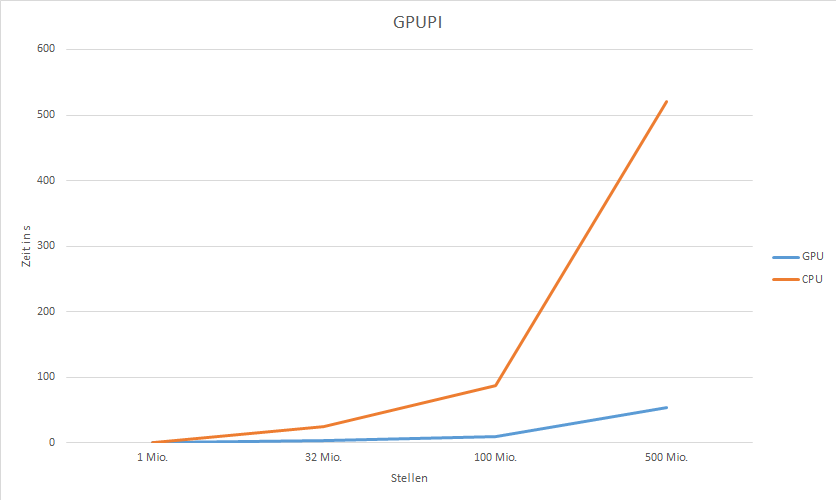
\includegraphics[width=17cm]{images/gpupi.png}
		\caption{GPUPI-Benchmark}
	\end{center}
\end{figure}
\newpage
\subsubsection{Fazit}
Durch diese spezielle parallele Implementierung und des gewählten Algorithmus werden nur die nächsten 9 Stellen von Pi nach zum Beispiel der 1 Milliardsten ausgegeben. Auch hier liegt die GPU ab mehreren 10 Mio Stellen klar im Vorteil.